\chapter{System Design}
\label{chapter:design}

\section{Overview}
    \begin{figure}[htb]
        \centering
        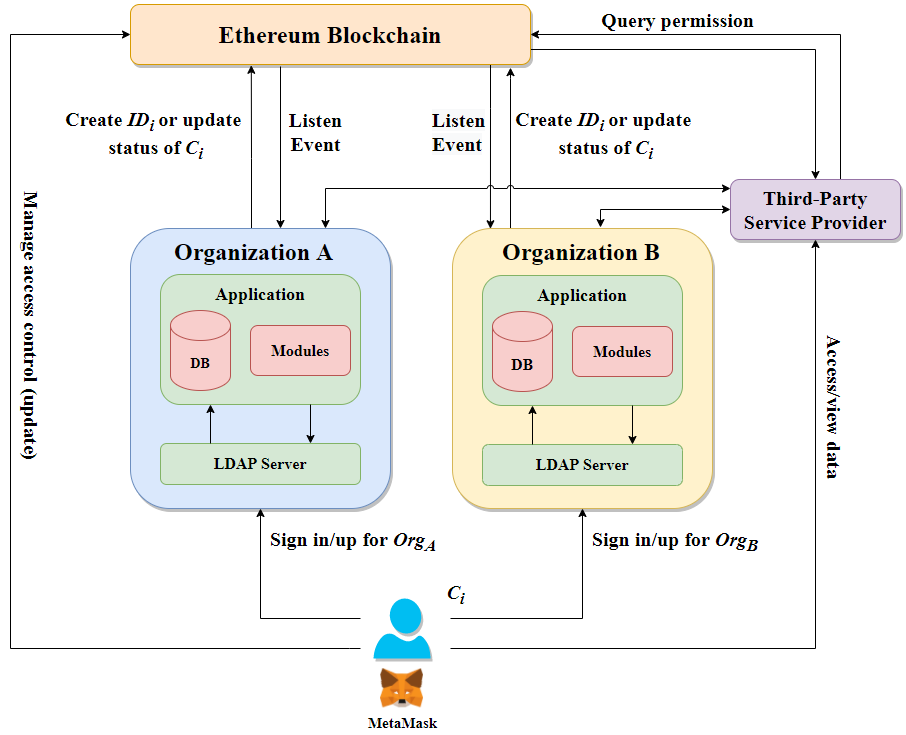
\includegraphics[height=!,width=1\linewidth,keepaspectratio=true]{figures/system_architecture.png}
        \caption{{\footnotesize System Architecture}}
        \label{fig:system_architecture}
    \end{figure}
    The architecture of our system is given in figure~\ref{fig:system_architecture}. Our proposed system solved the account integration and identity verification. And it can apply to various scenarios which need data sharing and distributed access control management such as open banking, medical records, and academic records. At the initial stage, every organization and TSP get an Ethereum address and its corresponding private key to take part in this ecosystem. They must keep their private key safe, or identity theft may occur.  There are several parties in our system: blockchain network, organization, third-party service provider, and user. The interpretation of these parties is stated as following:\par

    \begin{itemize}
        \item \textbf{Blockchain network:} The Ethereum blockchain network is responsible for the user's digital identity and access control management through smart contracts, including identity creation and storage. There have two kinds of contracts to realize that account integration and access manager, detailed in Sect.~\ref{chapter:implementation}.  
        \item \textbf{Organization:} A set of organizations within an ecosystem, identified by the Ethereum account and IP addresses. Each organization represents an independent system, it owns membership software that provides an organization with functionality such as storing and editing member information. The organization not only provides services to customers depend on applications, but also collects user data by using a database. In this paper, organizations provide an interface that users decide to share data.
        \item \textbf{Third-party service provider:} The third-party service provider can be any organization or entity that performs financial services to customer. In this paper, we assume that TSP doesn't manage membership software and they retrieve customer data through blockchain technology.
        \item \textbf{User:} A user owns an organization account and wants to participate in our proposed system. After registering an organization account, the user first needs to pass identity card authentication. Due to the digital identity is unique and important on the smart contract, the organization takes responsibility for ensuring the correct identification card number and the safety of user's personal data. Besides, the user should generate the Ethereum account themself through Metamask.
    \end{itemize}

    \newpage    
\section{Scenario}
    \begin{figure}[htb]
        \centering
        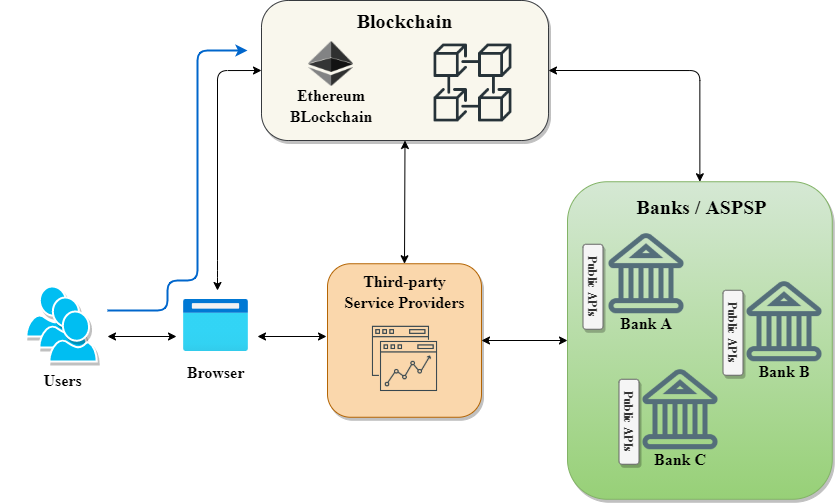
\includegraphics[height=!,width=1\linewidth,keepaspectratio=true]{figures/system architecture-banks.png}
        \caption{{\footnotesize Relation between open banking roles}}
        \label{fig:relation}
    \end{figure}
        From the user perspective, our proposed system provides a single digital identity and access control. The access control for data sharing is constructed using smart contracts. So when banks disclose user's personal data to TSP, banks must have the user's consent through call specific user's smart contract. \par
        In order to apply our proposed system to open banking ecosystem, we have three clearly defined roles: Customer (User), Financial institution, and Third-party services provider. Figure~\ref{fig:relation} gives an overview of our proposed system. It shows the relation between these roles and includes workflows, detailed in Sect.~\ref{ssec:workflow} Each customer interacts with Blockchain by using MetaMask, they not only login with MetaMask but also manage their own access manager contract. That's why customers can allow the specific party to access their data.
    
\section{Workflow} \label{ssec:workflow}
    \subsection{Identity verification}
    \subsection{Account binding}
    \subsection{Third-party login with Ethereum account}
    \subsection{Data sharing}